% Options for packages loaded elsewhere
\PassOptionsToPackage{unicode}{hyperref}
\PassOptionsToPackage{hyphens}{url}
%
\documentclass[
]{article}
\usepackage{amsmath,amssymb}
\usepackage{lmodern}
\usepackage{iftex}
\ifPDFTeX
  \usepackage[T1]{fontenc}
  \usepackage[utf8]{inputenc}
  \usepackage{textcomp} % provide euro and other symbols
\else % if luatex or xetex
  \usepackage{unicode-math}
  \defaultfontfeatures{Scale=MatchLowercase}
  \defaultfontfeatures[\rmfamily]{Ligatures=TeX,Scale=1}
\fi
% Use upquote if available, for straight quotes in verbatim environments
\IfFileExists{upquote.sty}{\usepackage{upquote}}{}
\IfFileExists{microtype.sty}{% use microtype if available
  \usepackage[]{microtype}
  \UseMicrotypeSet[protrusion]{basicmath} % disable protrusion for tt fonts
}{}
\makeatletter
\@ifundefined{KOMAClassName}{% if non-KOMA class
  \IfFileExists{parskip.sty}{%
    \usepackage{parskip}
  }{% else
    \setlength{\parindent}{0pt}
    \setlength{\parskip}{6pt plus 2pt minus 1pt}}
}{% if KOMA class
  \KOMAoptions{parskip=half}}
\makeatother
\usepackage{xcolor}
\IfFileExists{xurl.sty}{\usepackage{xurl}}{} % add URL line breaks if available
\IfFileExists{bookmark.sty}{\usepackage{bookmark}}{\usepackage{hyperref}}
\hypersetup{
  pdftitle={Laboratorio 2 IN5602 - Semestre Otoño 2021},
  pdfauthor={Nicolás Acevedo, Constanza Bastías y Pablo Ubilla},
  hidelinks,
  pdfcreator={LaTeX via pandoc}}
\urlstyle{same} % disable monospaced font for URLs
\usepackage[margin=1in]{geometry}
\usepackage{color}
\usepackage{fancyvrb}
\newcommand{\VerbBar}{|}
\newcommand{\VERB}{\Verb[commandchars=\\\{\}]}
\DefineVerbatimEnvironment{Highlighting}{Verbatim}{commandchars=\\\{\}}
% Add ',fontsize=\small' for more characters per line
\usepackage{framed}
\definecolor{shadecolor}{RGB}{248,248,248}
\newenvironment{Shaded}{\begin{snugshade}}{\end{snugshade}}
\newcommand{\AlertTok}[1]{\textcolor[rgb]{0.94,0.16,0.16}{#1}}
\newcommand{\AnnotationTok}[1]{\textcolor[rgb]{0.56,0.35,0.01}{\textbf{\textit{#1}}}}
\newcommand{\AttributeTok}[1]{\textcolor[rgb]{0.77,0.63,0.00}{#1}}
\newcommand{\BaseNTok}[1]{\textcolor[rgb]{0.00,0.00,0.81}{#1}}
\newcommand{\BuiltInTok}[1]{#1}
\newcommand{\CharTok}[1]{\textcolor[rgb]{0.31,0.60,0.02}{#1}}
\newcommand{\CommentTok}[1]{\textcolor[rgb]{0.56,0.35,0.01}{\textit{#1}}}
\newcommand{\CommentVarTok}[1]{\textcolor[rgb]{0.56,0.35,0.01}{\textbf{\textit{#1}}}}
\newcommand{\ConstantTok}[1]{\textcolor[rgb]{0.00,0.00,0.00}{#1}}
\newcommand{\ControlFlowTok}[1]{\textcolor[rgb]{0.13,0.29,0.53}{\textbf{#1}}}
\newcommand{\DataTypeTok}[1]{\textcolor[rgb]{0.13,0.29,0.53}{#1}}
\newcommand{\DecValTok}[1]{\textcolor[rgb]{0.00,0.00,0.81}{#1}}
\newcommand{\DocumentationTok}[1]{\textcolor[rgb]{0.56,0.35,0.01}{\textbf{\textit{#1}}}}
\newcommand{\ErrorTok}[1]{\textcolor[rgb]{0.64,0.00,0.00}{\textbf{#1}}}
\newcommand{\ExtensionTok}[1]{#1}
\newcommand{\FloatTok}[1]{\textcolor[rgb]{0.00,0.00,0.81}{#1}}
\newcommand{\FunctionTok}[1]{\textcolor[rgb]{0.00,0.00,0.00}{#1}}
\newcommand{\ImportTok}[1]{#1}
\newcommand{\InformationTok}[1]{\textcolor[rgb]{0.56,0.35,0.01}{\textbf{\textit{#1}}}}
\newcommand{\KeywordTok}[1]{\textcolor[rgb]{0.13,0.29,0.53}{\textbf{#1}}}
\newcommand{\NormalTok}[1]{#1}
\newcommand{\OperatorTok}[1]{\textcolor[rgb]{0.81,0.36,0.00}{\textbf{#1}}}
\newcommand{\OtherTok}[1]{\textcolor[rgb]{0.56,0.35,0.01}{#1}}
\newcommand{\PreprocessorTok}[1]{\textcolor[rgb]{0.56,0.35,0.01}{\textit{#1}}}
\newcommand{\RegionMarkerTok}[1]{#1}
\newcommand{\SpecialCharTok}[1]{\textcolor[rgb]{0.00,0.00,0.00}{#1}}
\newcommand{\SpecialStringTok}[1]{\textcolor[rgb]{0.31,0.60,0.02}{#1}}
\newcommand{\StringTok}[1]{\textcolor[rgb]{0.31,0.60,0.02}{#1}}
\newcommand{\VariableTok}[1]{\textcolor[rgb]{0.00,0.00,0.00}{#1}}
\newcommand{\VerbatimStringTok}[1]{\textcolor[rgb]{0.31,0.60,0.02}{#1}}
\newcommand{\WarningTok}[1]{\textcolor[rgb]{0.56,0.35,0.01}{\textbf{\textit{#1}}}}
\usepackage{longtable,booktabs,array}
\usepackage{calc} % for calculating minipage widths
% Correct order of tables after \paragraph or \subparagraph
\usepackage{etoolbox}
\makeatletter
\patchcmd\longtable{\par}{\if@noskipsec\mbox{}\fi\par}{}{}
\makeatother
% Allow footnotes in longtable head/foot
\IfFileExists{footnotehyper.sty}{\usepackage{footnotehyper}}{\usepackage{footnote}}
\makesavenoteenv{longtable}
\usepackage{graphicx}
\makeatletter
\def\maxwidth{\ifdim\Gin@nat@width>\linewidth\linewidth\else\Gin@nat@width\fi}
\def\maxheight{\ifdim\Gin@nat@height>\textheight\textheight\else\Gin@nat@height\fi}
\makeatother
% Scale images if necessary, so that they will not overflow the page
% margins by default, and it is still possible to overwrite the defaults
% using explicit options in \includegraphics[width, height, ...]{}
\setkeys{Gin}{width=\maxwidth,height=\maxheight,keepaspectratio}
% Set default figure placement to htbp
\makeatletter
\def\fps@figure{htbp}
\makeatother
\setlength{\emergencystretch}{3em} % prevent overfull lines
\providecommand{\tightlist}{%
  \setlength{\itemsep}{0pt}\setlength{\parskip}{0pt}}
\setcounter{secnumdepth}{-\maxdimen} % remove section numbering
\ifLuaTeX
  \usepackage{selnolig}  % disable illegal ligatures
\fi

\title{Laboratorio 2 IN5602 - Semestre Otoño 2021}
\author{Nicolás Acevedo, Constanza Bastías y Pablo Ubilla}
\date{14 de abril de 2021}

\begin{document}
\maketitle

{
\setcounter{tocdepth}{2}
\tableofcontents
}
\hypertarget{machine-learning}{%
\section{Machine Learning}\label{machine-learning}}

Modelos que puedan automáticamente aprender sobre conjuntos de datos y
su forma funcional. Se puede utiliar un conjunto determinado de
características para entrenar un algoritmo y extraer información. Estos
algoritmos pueden clasificarse según la cantidad y el tipo de
supervisión durante el entrenamiento. Los dos tipos principales en los
que se enfoca el curso son:

\begin{enumerate}
\def\labelenumi{\arabic{enumi}.}
\tightlist
\item
  Learners supervisados: construyen modelos predictivos.
\item
  Learners no supervisados: construyen modelos descriptivos.
\end{enumerate}

\textbf{¿Cuándo usar ML?}

\begin{enumerate}
\def\labelenumi{\arabic{enumi}.}
\tightlist
\item
  Foco en el pronóstico y no en el entendimiento de las relaciones de
  las variables.
\item
  Cuando existen relaciones complejas y no lineales.
\item
  Base de datos ``grandes''
\end{enumerate}

\hypertarget{aprendizaje-supervisado}{%
\subsection{Aprendizaje supervisado}\label{aprendizaje-supervisado}}

El algoritmo intenta modelar las relaciones entre la variable objetivo
(variable que se predice, \(Y\)) y los atributos (variables predictoras,
\(X's\)). Por ejemplo: usar los atributos de una casa (\(X's\)) para
predecir el precio de venta (\(Y\))

La mayoría de los problemas de aprendizaje supervisado pueden agruparse
en regresión o clasificación.

\begin{enumerate}
\def\labelenumi{\alph{enumi})}
\tightlist
\item
  Cuando el objetivo es predecir un resultado numérico, nos referimos a
  un problema de regresión (no debe confundirse con el modelo de
  regresión lineal).
\item
  Cuando el objetivo es predecir un resultado categórico, nos referimos
  a un problema de clasificación.
\end{enumerate}

\hypertarget{aprendizaje-sin-supervisiuxf3n}{%
\subsection{Aprendizaje sin
supervisión}\label{aprendizaje-sin-supervisiuxf3n}}

El objetivo es describir los datos, pero a el análisis se realiza sin
una variable objetivo (\(Y\)). El aprendizaje no supervisado se ocupa de
identificar grupos en un conjunto de datos. Los grupos pueden estar
definidos por las unidades (clustering) o por las características.

\hypertarget{divisiuxf3n-de-los-datos}{%
\subsection{División de los datos}\label{divisiuxf3n-de-los-datos}}

Para dividir los datos podemos usar muestreo aleatorio (Por lo general,
se divide haciendo ``80-20''o ``70-30'')

\begin{itemize}
\item
  Data train: Estos datos se utilizan para desarrollar conjuntos de
  características, entrenar el algoritmo, comparar modelos.
\item
  Data test: Estos datos se utilizan para estimar una evaluación
  imparcial del rendimiento del modelo.
\end{itemize}

\hypertarget{desarollo-del-laboratorio}{%
\section{Desarollo del laboratorio}\label{desarollo-del-laboratorio}}

\hypertarget{enunciado}{%
\subsection{Enunciado}\label{enunciado}}

Se tiene información sobre ventas de propiedades en EE.UU y se requiere
utilizar los atributos de estas propiedades para predecir el precio de
venta de la vivienda.

\begin{itemize}
\tightlist
\item
  Tipo de problema: regresión supervisada (\(Y\) es númerico)
\item
  Resultado de interés: \texttt{Sale\_Price} (en dólares)
\item
  Características o variables explicativas \(X\): 80
\item
  Observaciones: 2.930
\end{itemize}

\begin{Shaded}
\begin{Highlighting}[]
\FunctionTok{rm}\NormalTok{(}\AttributeTok{list=}\FunctionTok{ls}\NormalTok{())                }\CommentTok{\#Limpia todos los objetos creados en R}
\FunctionTok{graphics.off}\NormalTok{()           }\CommentTok{\#Limpia los gráficos}
\FunctionTok{options}\NormalTok{(}\AttributeTok{digits =} \DecValTok{3}\NormalTok{)  }\CommentTok{\#Dígitos después del punto para observar (décimas, centésimas,...)}
\FunctionTok{set.seed}\NormalTok{(}\DecValTok{12345}\NormalTok{)      }\CommentTok{\#Fijar semilla de aleatoriedad}
\CommentTok{\# setwd("C:/Users/color/Downloads/Marketing/LAB2\_IN5602") \#Fijar directorio de preferencia}
\end{Highlighting}
\end{Shaded}

\hypertarget{paquetes}{%
\subsubsection{Paquetes}\label{paquetes}}

\begin{Shaded}
\begin{Highlighting}[]
\FunctionTok{library}\NormalTok{(readr)     }\CommentTok{\#Para leer CSV}
\FunctionTok{library}\NormalTok{(glmnet)    }\CommentTok{\#Para ajustar modelo lineal}
\FunctionTok{library}\NormalTok{(corrplot)  }\CommentTok{\#Para realizar correlogramas}
\FunctionTok{library}\NormalTok{(dplyr)     }\CommentTok{\#Para manipulación de datos}
\FunctionTok{library}\NormalTok{(ggplot2)   }\CommentTok{\#Para gráficos}
\FunctionTok{library}\NormalTok{(caret)     }\CommentTok{\#Para validar y entrenar los modelos}
\FunctionTok{library}\NormalTok{(knitr) }
\end{Highlighting}
\end{Shaded}

\hypertarget{carga-de-datos}{%
\subsubsection{Carga de datos}\label{carga-de-datos}}

\begin{Shaded}
\begin{Highlighting}[]
\NormalTok{Casas }\OtherTok{\textless{}{-}} \FunctionTok{read.csv}\NormalTok{(}\StringTok{"Casas.csv"}\NormalTok{)}
\FunctionTok{kable}\NormalTok{(Casas[}\DecValTok{1}\SpecialCharTok{:}\DecValTok{5}\NormalTok{,}\DecValTok{1}\SpecialCharTok{:}\DecValTok{9}\NormalTok{]) }\CommentTok{\#kable crea una tabla head(Casas) sirve para visualiar la data}
\end{Highlighting}
\end{Shaded}

\begin{longtable}[]{@{}
  >{\raggedleft\arraybackslash}p{(\columnwidth - 16\tabcolsep) * \real{0.02}}
  >{\raggedright\arraybackslash}p{(\columnwidth - 16\tabcolsep) * \real{0.26}}
  >{\raggedright\arraybackslash}p{(\columnwidth - 16\tabcolsep) * \real{0.18}}
  >{\raggedleft\arraybackslash}p{(\columnwidth - 16\tabcolsep) * \real{0.09}}
  >{\raggedleft\arraybackslash}p{(\columnwidth - 16\tabcolsep) * \real{0.06}}
  >{\raggedright\arraybackslash}p{(\columnwidth - 16\tabcolsep) * \real{0.05}}
  >{\raggedright\arraybackslash}p{(\columnwidth - 16\tabcolsep) * \real{0.11}}
  >{\raggedright\arraybackslash}p{(\columnwidth - 16\tabcolsep) * \real{0.13}}
  >{\raggedright\arraybackslash}p{(\columnwidth - 16\tabcolsep) * \real{0.09}}@{}}
\toprule
X & MS\_SubClass & MS\_Zoning & Lot\_Frontage & Lot\_Area & Street &
Alley & Lot\_Shape & Land\_Contour \\
\midrule
\endhead
1 & One\_Story\_1946\_and\_Newer\_All\_Styles &
Residential\_Low\_Density & 141 & 31770 & Pave & No\_Alley\_Access &
Slightly\_Irregular & Lvl \\
2 & One\_Story\_1946\_and\_Newer\_All\_Styles &
Residential\_High\_Density & 80 & 11622 & Pave & No\_Alley\_Access &
Regular & Lvl \\
3 & One\_Story\_1946\_and\_Newer\_All\_Styles &
Residential\_Low\_Density & 81 & 14267 & Pave & No\_Alley\_Access &
Slightly\_Irregular & Lvl \\
4 & One\_Story\_1946\_and\_Newer\_All\_Styles &
Residential\_Low\_Density & 93 & 11160 & Pave & No\_Alley\_Access &
Regular & Lvl \\
5 & Two\_Story\_1946\_and\_Newer & Residential\_Low\_Density & 74 &
13830 & Pave & No\_Alley\_Access & Slightly\_Irregular & Lvl \\
\bottomrule
\end{longtable}

\hypertarget{divisiuxf3n-de-los-datos-1}{%
\subsubsection{División de los datos}\label{divisiuxf3n-de-los-datos-1}}

Vamos a escoger 70\% entrenamiento y 30\% para testeo:

\begin{Shaded}
\begin{Highlighting}[]
\CommentTok{\# Construimos un vector que esta formado por números de filas aleatoriamente}
\NormalTok{index }\OtherTok{\textless{}{-}} \FunctionTok{sample}\NormalTok{(}\DecValTok{1}\SpecialCharTok{:}\FunctionTok{nrow}\NormalTok{(Casas), }\AttributeTok{size=} \FunctionTok{nrow}\NormalTok{(Casas)}\SpecialCharTok{*}\FloatTok{0.7}\NormalTok{)}
\CommentTok{\# Base de entrenamiento: del total de datos, tomamos las filas aletorizadas que tienen datos en index}
\NormalTok{train }\OtherTok{\textless{}{-}}\NormalTok{ Casas[index, ]}
\CommentTok{\# Anteponiendo el "{-}" escogemos las filas en de la base que no están en index }
\NormalTok{test  }\OtherTok{\textless{}{-}}\NormalTok{ Casas[}\SpecialCharTok{{-}}\NormalTok{index, ]}
\end{Highlighting}
\end{Shaded}

\hypertarget{eda}{%
\subsubsection{EDA}\label{eda}}

Antes de entrenar un modelo predictivo, o incluso antes de realizar
cualquier cálculo con un nuevo conjunto de datos, es muy importante
realizar una exploración descriptiva de los mismos. Este proceso permite
entender mejor que información contiene cada variable, así como detectar
posibles errores.

\hypertarget{gruxe1ficos}{%
\paragraph{Gráficos}\label{gruxe1ficos}}

\hypertarget{variable-de-interuxe9s}{%
\paragraph{Variable de interés}\label{variable-de-interuxe9s}}

\begin{Shaded}
\begin{Highlighting}[]
\FunctionTok{ggplot}\NormalTok{(}\AttributeTok{data=}\NormalTok{Casas)}\SpecialCharTok{+} \CommentTok{\#Se define un gráfico con ggplot()}
  \FunctionTok{aes}\NormalTok{(}\AttributeTok{x=}\NormalTok{Sale\_Price)}\SpecialCharTok{+} \CommentTok{\#Solo le ingresamos el eje "x" para un histograma}
  \FunctionTok{geom\_histogram}\NormalTok{(}\AttributeTok{col=}\StringTok{"black"}\NormalTok{, }\AttributeTok{fill=}\StringTok{"green"}\NormalTok{, }\AttributeTok{alpha =} \FloatTok{0.2}\NormalTok{) }\CommentTok{\# Se define la forma del gráfico. "col" pinta el contorno, "fill" el entorno y "alpha" entrega transparencia }
\end{Highlighting}
\end{Shaded}

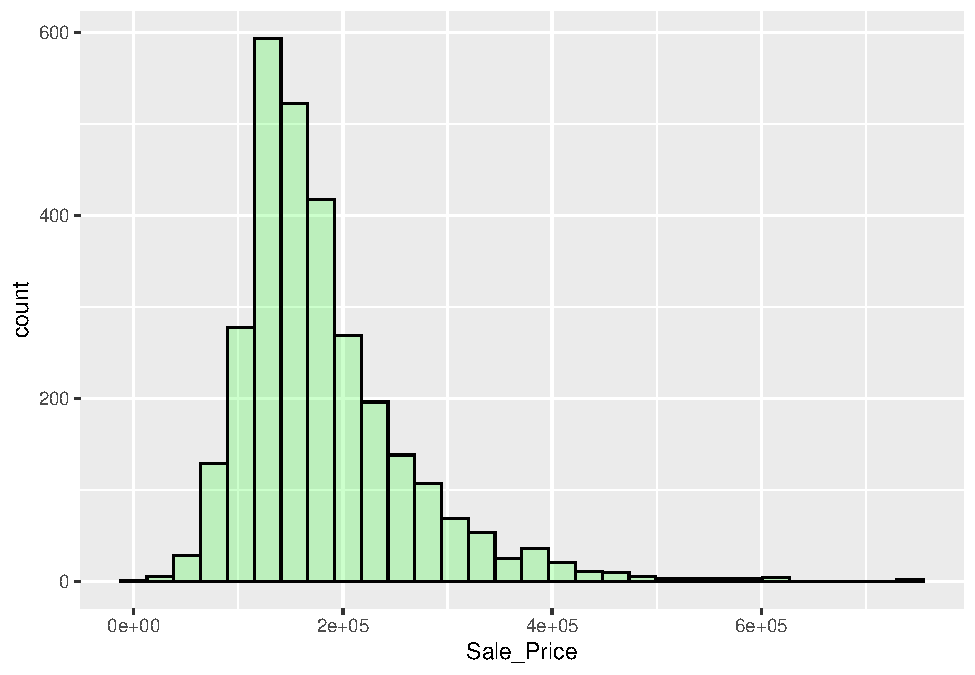
\includegraphics{LAB02_files/figure-latex/histograma-1.pdf}

\begin{Shaded}
\begin{Highlighting}[]
\FunctionTok{ggplot}\NormalTok{(}\AttributeTok{data=}\NormalTok{Casas)}\SpecialCharTok{+}
  \FunctionTok{aes}\NormalTok{(}\AttributeTok{x=}\FunctionTok{log}\NormalTok{(Sale\_Price))}\SpecialCharTok{+}
  \FunctionTok{geom\_histogram}\NormalTok{(}\AttributeTok{col=}\StringTok{"black"}\NormalTok{, }\AttributeTok{fill=}\StringTok{"green"}\NormalTok{, }\AttributeTok{alpha=}\FloatTok{0.2}\NormalTok{)}\SpecialCharTok{+}
  \FunctionTok{xlab}\NormalTok{(}\StringTok{"Log(Precio de venta)"}\NormalTok{)}\SpecialCharTok{+} \CommentTok{\#Etiqueta para el eje x}
  \FunctionTok{ylab}\NormalTok{(}\StringTok{"Frecuencia"}\NormalTok{)}\SpecialCharTok{+} \CommentTok{\#Etiqueta para el eje y}
  \FunctionTok{ggtitle}\NormalTok{(}\StringTok{"Distribución log(Precio de venta)"}\NormalTok{)}\SpecialCharTok{+} \CommentTok{\#Título del gráfico}
  \FunctionTok{theme}\NormalTok{(}\AttributeTok{plot.title =} \FunctionTok{element\_text}\NormalTok{(}\AttributeTok{hjust =} \FloatTok{0.5}\NormalTok{)) }\CommentTok{\#centra el título en el gráfico. Lo ajusta en la posición horizontal (hjust = 0.5)}
\end{Highlighting}
\end{Shaded}

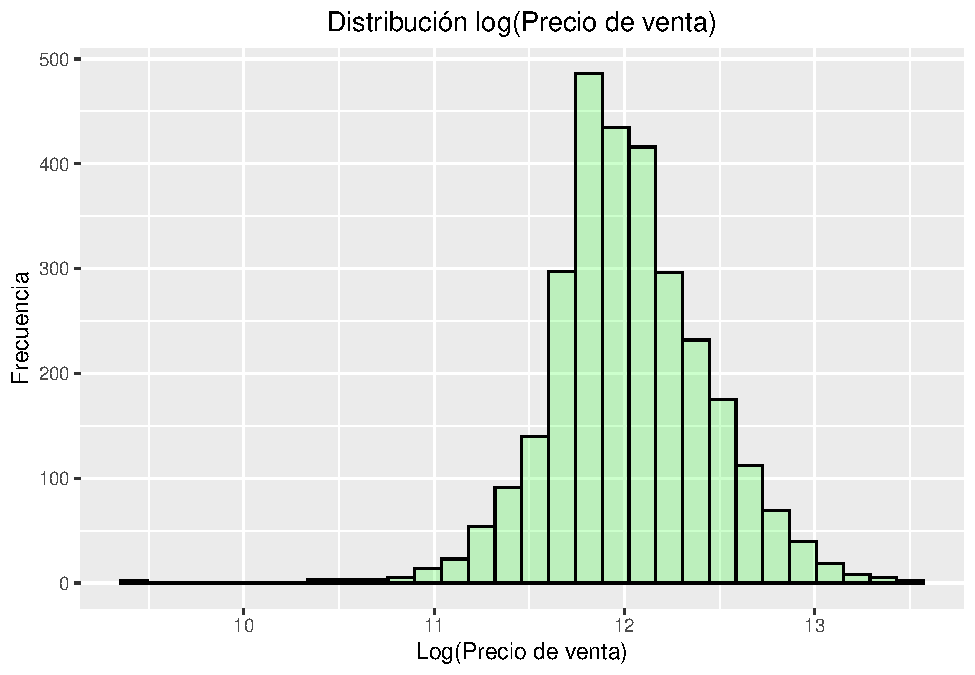
\includegraphics{LAB02_files/figure-latex/histograma 2-1.pdf}

\hypertarget{variables-explicativas}{%
\paragraph{Variables explicativas}\label{variables-explicativas}}

Escogemos algunas variables: \texttt{Year\_Built} (Año en que se
construyó la casa), \texttt{Roof\_Style} (Tipo de techo),
\texttt{Gr\_Liv\_Area} (espacio habitable total sobre el suelo de una
casa) y \texttt{Heating\_QC}(Calidad y estado de la calefacción)

\begin{Shaded}
\begin{Highlighting}[]
\CommentTok{\#R no siempre interpreta bien la naturaleza de las variables: Roof\_Style y Heating\_QC son factores, pero están como character(string)}

\CommentTok{\#en train}
\NormalTok{train}\SpecialCharTok{$}\NormalTok{Roof\_Style}\OtherTok{=}\FunctionTok{as.factor}\NormalTok{(train}\SpecialCharTok{$}\NormalTok{Roof\_Style)}
\NormalTok{train}\SpecialCharTok{$}\NormalTok{Heating\_QC}\OtherTok{=}\FunctionTok{as.factor}\NormalTok{(train}\SpecialCharTok{$}\NormalTok{Heating\_QC)}
\CommentTok{\#en test}
\NormalTok{test}\SpecialCharTok{$}\NormalTok{Roof\_Style}\OtherTok{=}\FunctionTok{as.factor}\NormalTok{(test}\SpecialCharTok{$}\NormalTok{Roof\_Style)}
\NormalTok{test}\SpecialCharTok{$}\NormalTok{Heating\_QC}\OtherTok{=}\FunctionTok{as.factor}\NormalTok{(test}\SpecialCharTok{$}\NormalTok{Heating\_QC)}
\end{Highlighting}
\end{Shaded}

\hypertarget{year_built}{%
\subparagraph{\texorpdfstring{\texttt{Year\_Built}}{Year\_Built}}\label{year_built}}

\begin{Shaded}
\begin{Highlighting}[]
\FunctionTok{library}\NormalTok{(gridExtra) }\CommentTok{\#Para unir gráficas}
\NormalTok{g1 }\OtherTok{\textless{}{-}} \FunctionTok{ggplot}\NormalTok{(Casas) }\SpecialCharTok{+}
  \FunctionTok{aes}\NormalTok{(}\AttributeTok{x=}\NormalTok{Year\_Built, }\AttributeTok{y=}\NormalTok{Sale\_Price) }\SpecialCharTok{+}
  \FunctionTok{geom\_point}\NormalTok{(}\AttributeTok{size=}\DecValTok{1}\NormalTok{, }\AttributeTok{alpha=}\FloatTok{0.4}\NormalTok{) }\SpecialCharTok{+} \CommentTok{\#"size" aumenta el tamaño de los puntos, "alpha" da transparencia}
  \FunctionTok{geom\_smooth}\NormalTok{(}\AttributeTok{se=}\ConstantTok{FALSE}\NormalTok{) }\SpecialCharTok{+} \CommentTok{\#Agregamos un ajuste no lineal sobre los puntos. "se" integra errores estándares}
  \FunctionTok{xlab}\NormalTok{(}\StringTok{"Año de construcción"}\NormalTok{)}


\NormalTok{g2 }\OtherTok{\textless{}{-}} \FunctionTok{ggplot}\NormalTok{(Casas) }\SpecialCharTok{+}
  \FunctionTok{aes}\NormalTok{(}\AttributeTok{x=}\NormalTok{Year\_Built, }\AttributeTok{y=}\NormalTok{Sale\_Price) }\SpecialCharTok{+}
  \FunctionTok{geom\_point}\NormalTok{(}\AttributeTok{size =} \DecValTok{1}\NormalTok{, }\AttributeTok{alpha =}\NormalTok{ .}\DecValTok{4}\NormalTok{) }\SpecialCharTok{+} 
  \FunctionTok{geom\_smooth}\NormalTok{(}\AttributeTok{method =} \StringTok{"lm"}\NormalTok{, }\AttributeTok{se =} \ConstantTok{FALSE}\NormalTok{) }\SpecialCharTok{+} \CommentTok{\#Agregamos un ajuste lineal sobre los puntos.}
  \FunctionTok{scale\_y\_log10}\NormalTok{() }\SpecialCharTok{+} \CommentTok{\# "scale\_y\_log10" transforma el eje "y" a logaritmo.}
  \FunctionTok{xlab}\NormalTok{(}\StringTok{"Año de construcción"}\NormalTok{) }

\FunctionTok{grid.arrange}\NormalTok{(g1, g2, }\AttributeTok{nrow =} \DecValTok{1}\NormalTok{) }\CommentTok{\#une las  gráficas. }
\end{Highlighting}
\end{Shaded}

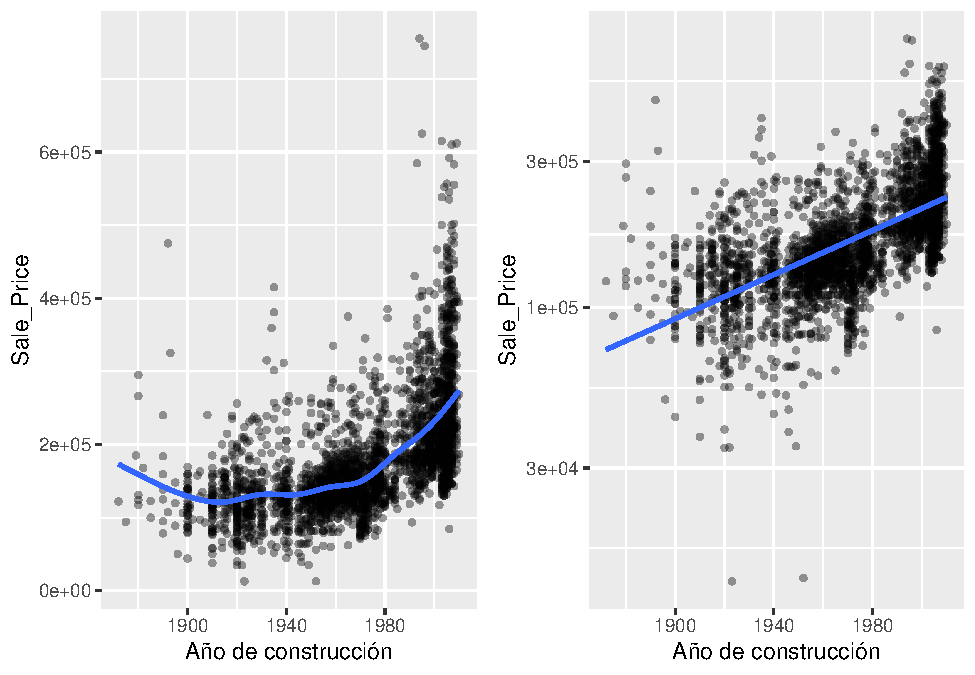
\includegraphics{LAB02_files/figure-latex/Gráfico de dispersión-1.pdf}

\hypertarget{gr_liv_area-seguxfan-heating_qc}{%
\subparagraph{\texorpdfstring{\texttt{Gr\_Liv\_Area} según
\texttt{Heating\_QC}}{Gr\_Liv\_Area según Heating\_QC}}\label{gr_liv_area-seguxfan-heating_qc}}

\begin{Shaded}
\begin{Highlighting}[]
\FunctionTok{ggplot}\NormalTok{(Casas) }\SpecialCharTok{+}
  \FunctionTok{aes}\NormalTok{(}\AttributeTok{x=}\NormalTok{Gr\_Liv\_Area, }\AttributeTok{y=}\NormalTok{Sale\_Price, }\AttributeTok{col=}\NormalTok{Heating\_QC)}\SpecialCharTok{+} \CommentTok{\#Se agrega una dimensión de colores "col".}
  \FunctionTok{geom\_point}\NormalTok{(}\AttributeTok{size=}\DecValTok{1}\NormalTok{, }\AttributeTok{alpha=}\FloatTok{0.4}\NormalTok{) }\SpecialCharTok{+}
  \FunctionTok{geom\_smooth}\NormalTok{(}\AttributeTok{se=}\ConstantTok{FALSE}\NormalTok{, }\AttributeTok{method=}\StringTok{"lm"}\NormalTok{) }\SpecialCharTok{+}
  \FunctionTok{xlab}\NormalTok{(}\StringTok{"Espacio habitable"}\NormalTok{) }
\end{Highlighting}
\end{Shaded}

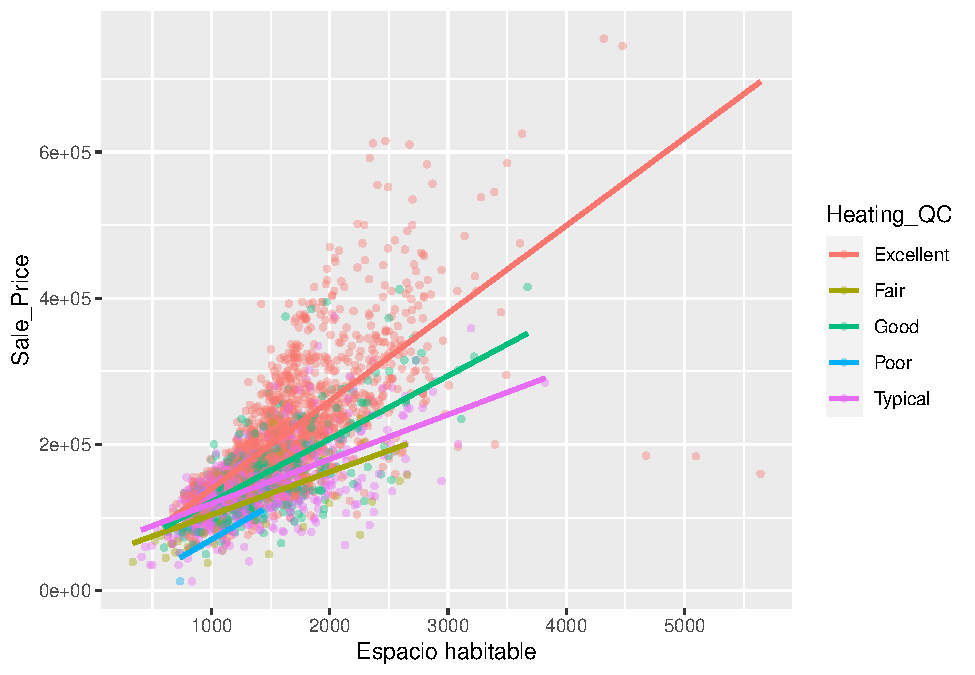
\includegraphics{LAB02_files/figure-latex/unnamed-chunk-1-1.pdf}

\hypertarget{roof_style}{%
\subparagraph{\texorpdfstring{\texttt{Roof\_Style}}{Roof\_Style}}\label{roof_style}}

\begin{Shaded}
\begin{Highlighting}[]
\FunctionTok{ggplot}\NormalTok{(Casas) }\SpecialCharTok{+}
  \FunctionTok{aes}\NormalTok{(}\AttributeTok{x=}\NormalTok{Roof\_Style, }\AttributeTok{y=}\FunctionTok{log}\NormalTok{(Sale\_Price)) }\SpecialCharTok{+}
  \FunctionTok{geom\_boxplot}\NormalTok{(}\AttributeTok{alpha=}\FloatTok{0.4}\NormalTok{, }\AttributeTok{fill=}\StringTok{"black"}\NormalTok{) }\CommentTok{\#cambiamos el tipo de gráfico}
\end{Highlighting}
\end{Shaded}

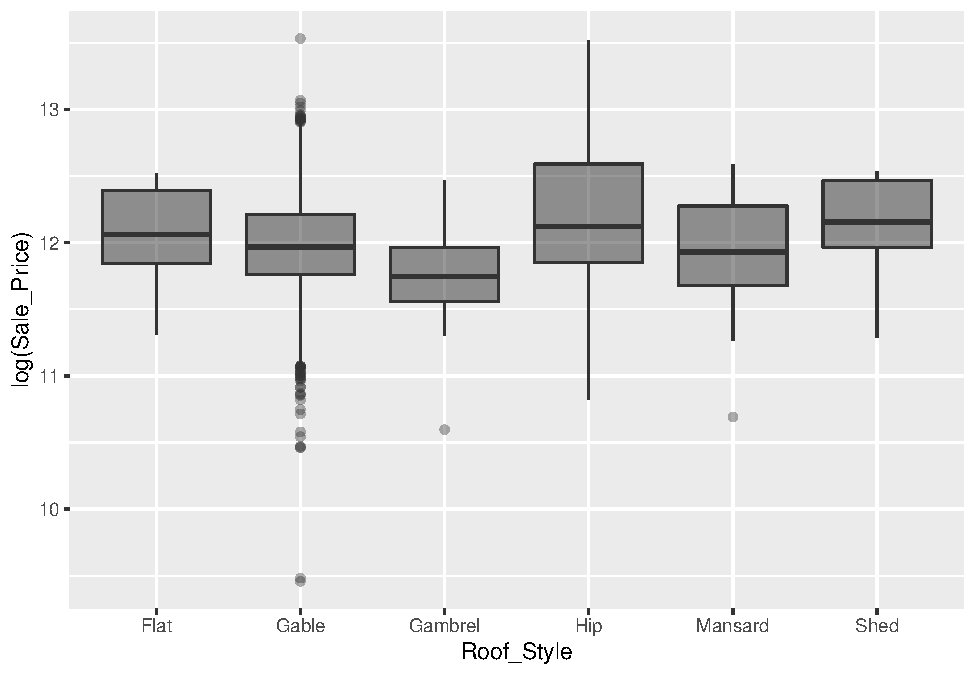
\includegraphics{LAB02_files/figure-latex/unnamed-chunk-2-1.pdf}

\hypertarget{regresiuxf3n-lineal}{%
\subsection{Regresión Lineal}\label{regresiuxf3n-lineal}}

\begin{Shaded}
\begin{Highlighting}[]
\NormalTok{train.lm }\OtherTok{\textless{}{-}} \FunctionTok{train}\NormalTok{(}\AttributeTok{form =}\NormalTok{ Sale\_Price }\SpecialCharTok{\textasciitilde{}}\NormalTok{ Year\_Built}\SpecialCharTok{+}\NormalTok{Gr\_Liv\_Area}\SpecialCharTok{+}\NormalTok{Roof\_Style}\SpecialCharTok{+}\NormalTok{Heating\_QC, }\CommentTok{\#Fórmula}
  \AttributeTok{data =}\NormalTok{ train, }\CommentTok{\#Datos}
  \AttributeTok{method =} \StringTok{"lm"}\NormalTok{, }\CommentTok{\#Algoritmo }
  \AttributeTok{trControl =} \FunctionTok{trainControl}\NormalTok{(}\AttributeTok{method =} \StringTok{"cv"}\NormalTok{, }\AttributeTok{number =} \DecValTok{5}\NormalTok{) }\CommentTok{\#Method = cross validation, number=10 (k{-}fold) }
\NormalTok{)}

\NormalTok{test.lm  }\OtherTok{\textless{}{-}} \FunctionTok{predict}\NormalTok{(train.lm , }\AttributeTok{newdata=}\NormalTok{test) }\CommentTok{\#Vector de datos predichos. Recibe una base de datos (newdata) y un modelo entrenado (train.lm)}
\NormalTok{error.lm }\OtherTok{\textless{}{-}}\NormalTok{ test}\SpecialCharTok{$}\NormalTok{Sale\_Price}\SpecialCharTok{{-}}\NormalTok{test.lm }\CommentTok{\#Calcular los errores de predicción (dato real {-} dato estimado)}
\end{Highlighting}
\end{Shaded}

\hypertarget{mars}{%
\subsection{MARS}\label{mars}}

Este algoritmo no asume una forma funcional de los datos, toma las
variables \(X\) y trata de ``formar'' funciones no lineales e
interacciones que se ajusten a los datos. Las no linealidades e
interacciones se van ``ajustando'' a una función escalonada o por tramos
donde el objetivo es encontrar puntos de cortes o ``knots'' que se
adecuan de mejor forma a los datos. Luego de haber de encontrado muchos
``knots'', el algoritmo realiza una ``limpieza'' donde se eliminan
puntos que no contribuyen significativamente a la precisión predictiva
(redundantes). Este proceso se le llama poda.

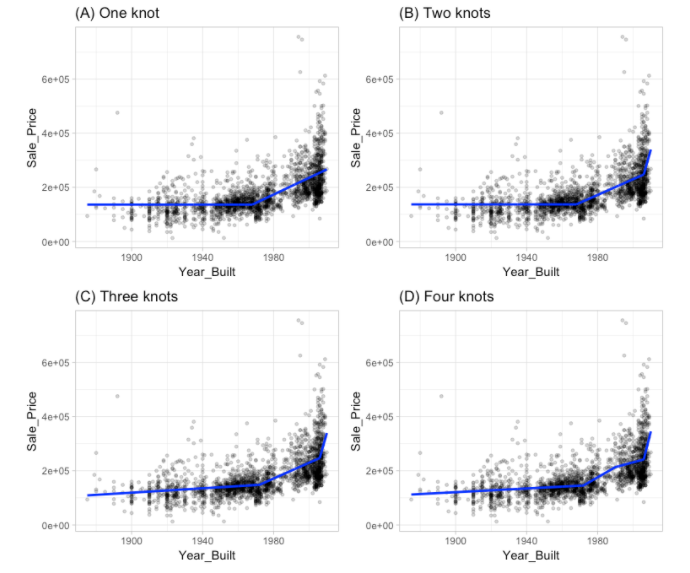
\includegraphics{3.png}

\begin{Shaded}
\begin{Highlighting}[]
\CommentTok{\#Ejecutar MARS (Multivariate adaptive regression spline)}
\NormalTok{train.mars }\OtherTok{\textless{}{-}} \FunctionTok{train}\NormalTok{(}\AttributeTok{form =}\NormalTok{ Sale\_Price }\SpecialCharTok{\textasciitilde{}}\NormalTok{ Year\_Built}\SpecialCharTok{+}\NormalTok{Gr\_Liv\_Area}\SpecialCharTok{+}\NormalTok{Roof\_Style}\SpecialCharTok{+}\NormalTok{Heating\_QC, }
                    \AttributeTok{data=}\NormalTok{train, }
                    \AttributeTok{method=}\StringTok{"earth"}\NormalTok{, }\CommentTok{\#MARS}
                    \AttributeTok{trControl =} \FunctionTok{trainControl}\NormalTok{(}\StringTok{"cv"}\NormalTok{, }\AttributeTok{number=}\DecValTok{5}\NormalTok{),}
                    \AttributeTok{preProcess =} \FunctionTok{c}\NormalTok{(}\StringTok{"center"}\NormalTok{,}\StringTok{"scale"}\NormalTok{), }\CommentTok{\#Pre{-}procesa datos. "center" resta el promedio de las variables, "scale" las divide por la desviación estandar. Esto ayuda para el tratamiento de outliers.}
                    \AttributeTok{tuneLength =} \DecValTok{5} \CommentTok{\#Indica que pruebe diferentes valores por default para el parámetro principal}
\NormalTok{)}
\FunctionTok{print}\NormalTok{(train.mars)}
\end{Highlighting}
\end{Shaded}

\begin{verbatim}
## Multivariate Adaptive Regression Spline 
## 
## 2051 samples
##    4 predictor
## 
## Pre-processing: centered (11), scaled (11) 
## Resampling: Cross-Validated (5 fold) 
## Summary of sample sizes: 1641, 1641, 1642, 1639, 1641 
## Resampling results across tuning parameters:
## 
##   nprune  RMSE   Rsquared  MAE  
##   2       56457  0.508     38925
##   3       47455  0.653     32511
##   5       47031  0.666     30742
##   6       45222  0.690     29631
##   8       44632  0.698     29577
## 
## Tuning parameter 'degree' was held constant at a value of 1
## RMSE was used to select the optimal model using the smallest value.
## The final values used for the model were nprune = 8 and degree = 1.
\end{verbatim}

\begin{Shaded}
\begin{Highlighting}[]
\FunctionTok{ggplot}\NormalTok{(train.mars)}
\end{Highlighting}
\end{Shaded}

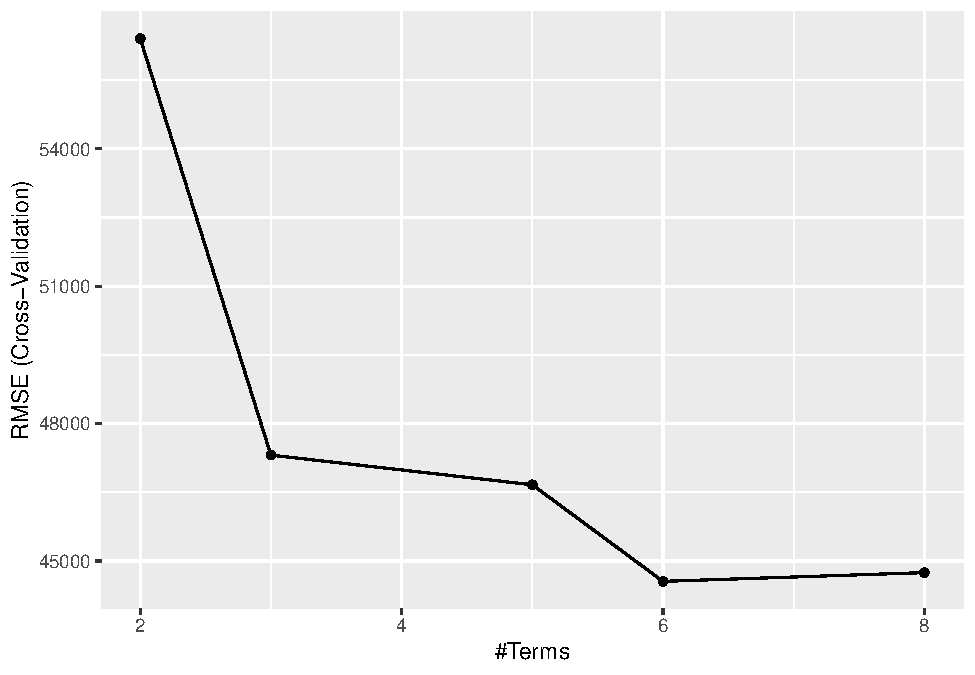
\includegraphics{LAB02_files/figure-latex/unnamed-chunk-4-1.pdf}

\begin{Shaded}
\begin{Highlighting}[]
\NormalTok{test.mars  }\OtherTok{\textless{}{-}} \FunctionTok{predict}\NormalTok{(train.mars, }\AttributeTok{newdata=}\NormalTok{test) }\CommentTok{\#Vector de datos predichos }
\NormalTok{error.mars }\OtherTok{\textless{}{-}}\NormalTok{ test}\SpecialCharTok{$}\NormalTok{Sale\_Price}\SpecialCharTok{{-}}\NormalTok{test.mars }\CommentTok{\#(dato real {-} dato estimado)}
\end{Highlighting}
\end{Shaded}

\hypertarget{k-nearest-neighbors}{%
\subsection{K-Nearest Neighbors}\label{k-nearest-neighbors}}

Es un algoritmo en el que cada observación se predice en función de su
``similitud'' con otras observaciones y luego usa el valor de respuesta
media de k observaciones como el resultado previsto. Para medir
``similitud'' usamos métricas (distancias) en el espacio
\(\mathcal{R}^j\). Para dos observaciones \(i\) y \(n\), \(J\)
predictores, tenemos la métricas:

\[\sqrt{\sum_{j=1}^J (X_{ij}-X_{nj})^2} \hspace{.5 cm} \text{(Métrica Eucliadiana)}\]

\[\sum_{j=1}^J |X_{ij}-X_{nj}| \hspace{.5 cm} \text{(Métrica Manhattan)}\]

\[\left(\sum_{j=1}^J |X_{ij}-X_{nj}|^{p}\right)^{1/p} \hspace{.5 cm} \text{(Métrica Minkowski)}\]
Al encontrar los k-vecinos más cercanos, ponderamos sus resultados
(\(Y\)):

\[\hat{Y}_i=w_1Y_{1,i}+...+w_kY_{k,i}\]

Si utilizamos ponderaciones \(w_k\) que no son iguales (ese caso es
\(w_k=1/k\)), puntos cercanos deberían pesar más que puntos lejanos.

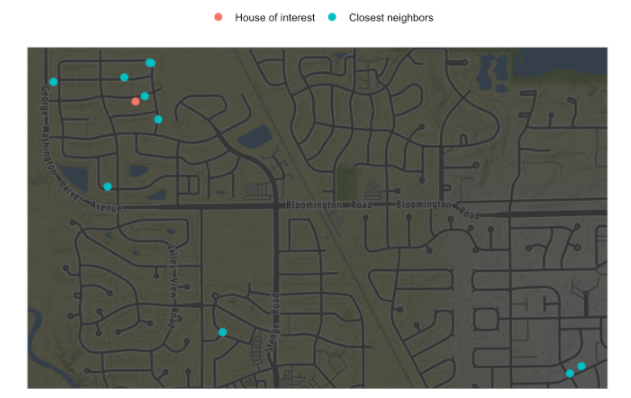
\includegraphics{4.png}

\begin{Shaded}
\begin{Highlighting}[]
\DocumentationTok{\#\#\# Ejecutar KNN}
\NormalTok{train.knn }\OtherTok{\textless{}{-}} \FunctionTok{train}\NormalTok{(Sale\_Price }\SpecialCharTok{\textasciitilde{}}\NormalTok{ Year\_Built}\SpecialCharTok{+}\NormalTok{Gr\_Liv\_Area}\SpecialCharTok{+}\NormalTok{Roof\_Style}\SpecialCharTok{+}\NormalTok{Heating\_QC, }
                   \AttributeTok{data=}\NormalTok{train, }\AttributeTok{method=}\StringTok{"knn"}\NormalTok{,  }
                   \AttributeTok{trControl =} \FunctionTok{trainControl}\NormalTok{(}\StringTok{"cv"}\NormalTok{, }\AttributeTok{number=}\DecValTok{5}\NormalTok{),}
                   \AttributeTok{preProcess =} \FunctionTok{c}\NormalTok{(}\StringTok{"center"}\NormalTok{,}\StringTok{"scale"}\NormalTok{),}
                   \AttributeTok{tuneLength =} \DecValTok{5} 
\NormalTok{)}

\FunctionTok{print}\NormalTok{(train.knn)}
\end{Highlighting}
\end{Shaded}

\begin{verbatim}
## k-Nearest Neighbors 
## 
## 2051 samples
##    4 predictor
## 
## Pre-processing: centered (11), scaled (11) 
## Resampling: Cross-Validated (5 fold) 
## Summary of sample sizes: 1639, 1642, 1641, 1641, 1641 
## Resampling results across tuning parameters:
## 
##   k   RMSE   Rsquared  MAE  
##    5  41606  0.737     27524
##    7  41355  0.737     27230
##    9  40698  0.746     26965
##   11  40571  0.747     26790
##   13  40758  0.744     26969
## 
## RMSE was used to select the optimal model using the smallest value.
## The final value used for the model was k = 11.
\end{verbatim}

\begin{Shaded}
\begin{Highlighting}[]
\FunctionTok{ggplot}\NormalTok{(train.knn)}
\end{Highlighting}
\end{Shaded}

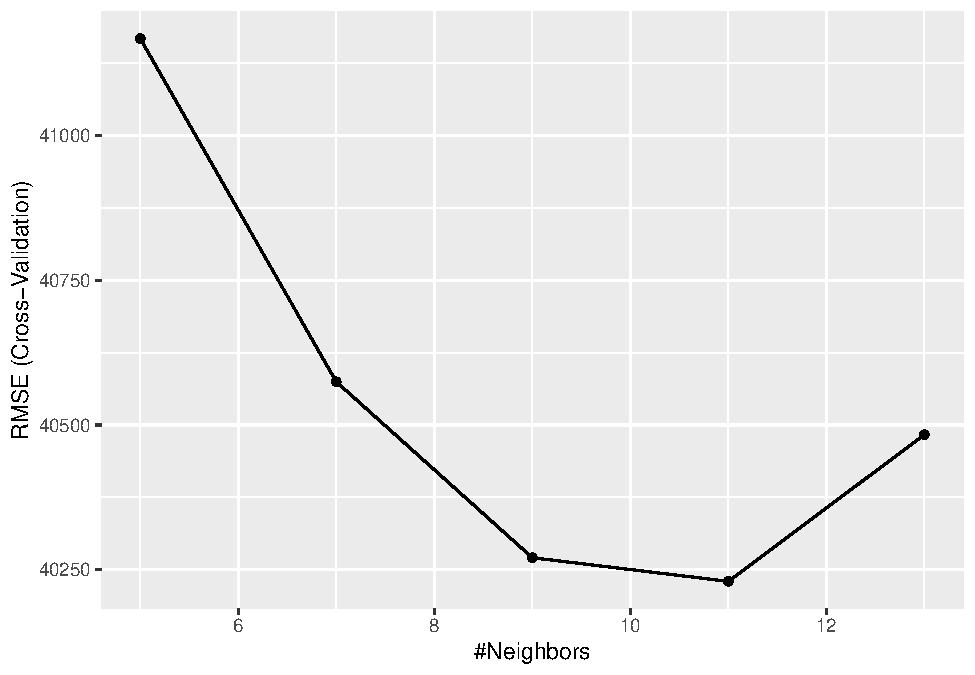
\includegraphics{LAB02_files/figure-latex/unnamed-chunk-5-1.pdf}

\begin{Shaded}
\begin{Highlighting}[]
\NormalTok{test.knn  }\OtherTok{\textless{}{-}} \FunctionTok{predict}\NormalTok{(train.knn, }\AttributeTok{newdata=}\NormalTok{test) }
\NormalTok{error.knn }\OtherTok{\textless{}{-}}\NormalTok{ test}\SpecialCharTok{$}\NormalTok{Sale\_Price}\SpecialCharTok{{-}}\NormalTok{test.knn}
\end{Highlighting}
\end{Shaded}

\hypertarget{cart}{%
\subsection{CART}\label{cart}}

Modelo basado en árboles de regresión - algoritmo no paramétrico - se
utiliza cuando hay múltiples regresores. Divide el espacio de las
características (\(X\)) según particiones binarias dada alguna regla de
condición. De esto van resultando regiones más pequeñas.

El objetivo en cada nodo es encontrar la ``mejor'' característica
(\(X_j\)) para dividir los datos restantes en una de dos regiones
(\(R_1\) y \(R_2\)) de manera que el error general entre la respuesta
real (\(Y\)) y la constante predicha (\(c\)) se minimiza. Para problemas
de regresión, la función objetivo a minimizar es el \(SSE\) (suma de
cuadrados residuales) total.

\[SSE=\sum_{i\in R_1} (y_i-c_1)^2 + \sum_{i\in R_2} (y_i-c_2)^2 \]
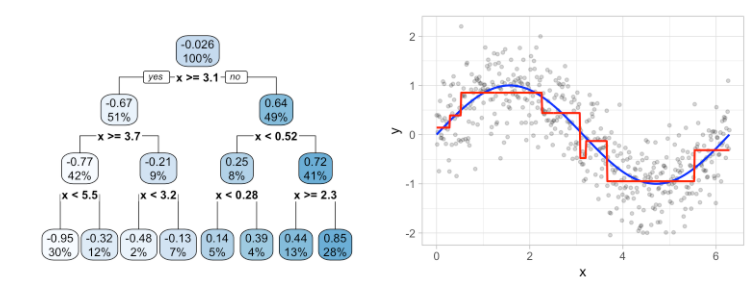
\includegraphics{5.png}

\begin{Shaded}
\begin{Highlighting}[]
\DocumentationTok{\#\#\# Ejecutar CART (Classification and Regression Trees)}
\NormalTok{train.cart }\OtherTok{\textless{}{-}} \FunctionTok{train}\NormalTok{(Sale\_Price }\SpecialCharTok{\textasciitilde{}}\NormalTok{ Year\_Built}\SpecialCharTok{+}\NormalTok{Gr\_Liv\_Area}\SpecialCharTok{+}\NormalTok{Roof\_Style}\SpecialCharTok{+}\NormalTok{Heating\_QC, }
                    \AttributeTok{data=}\NormalTok{train, }\AttributeTok{method=}\StringTok{"rpart2"}\NormalTok{,  }
                    \AttributeTok{trControl =} \FunctionTok{trainControl}\NormalTok{(}\StringTok{"cv"}\NormalTok{, }\AttributeTok{number=}\DecValTok{5}\NormalTok{),}
                    \AttributeTok{preProcess =} \FunctionTok{c}\NormalTok{(}\StringTok{"center"}\NormalTok{,}\StringTok{"scale"}\NormalTok{),}
                    \AttributeTok{tuneLength =} \DecValTok{5}
\NormalTok{)}
\FunctionTok{print}\NormalTok{(train.cart)}
\end{Highlighting}
\end{Shaded}

\begin{verbatim}
## CART 
## 
## 2051 samples
##    4 predictor
## 
## Pre-processing: centered (11), scaled (11) 
## Resampling: Cross-Validated (5 fold) 
## Summary of sample sizes: 1641, 1641, 1641, 1640, 1641 
## Resampling results across tuning parameters:
## 
##   maxdepth  RMSE   Rsquared  MAE  
##   1         64280  0.362     44313
##   2         55602  0.527     38800
##   3         54264  0.550     38025
##   4         52028  0.587     36498
##   5         46730  0.668     32660
## 
## RMSE was used to select the optimal model using the smallest value.
## The final value used for the model was maxdepth = 5.
\end{verbatim}

\begin{Shaded}
\begin{Highlighting}[]
\FunctionTok{ggplot}\NormalTok{(train.cart)}
\end{Highlighting}
\end{Shaded}

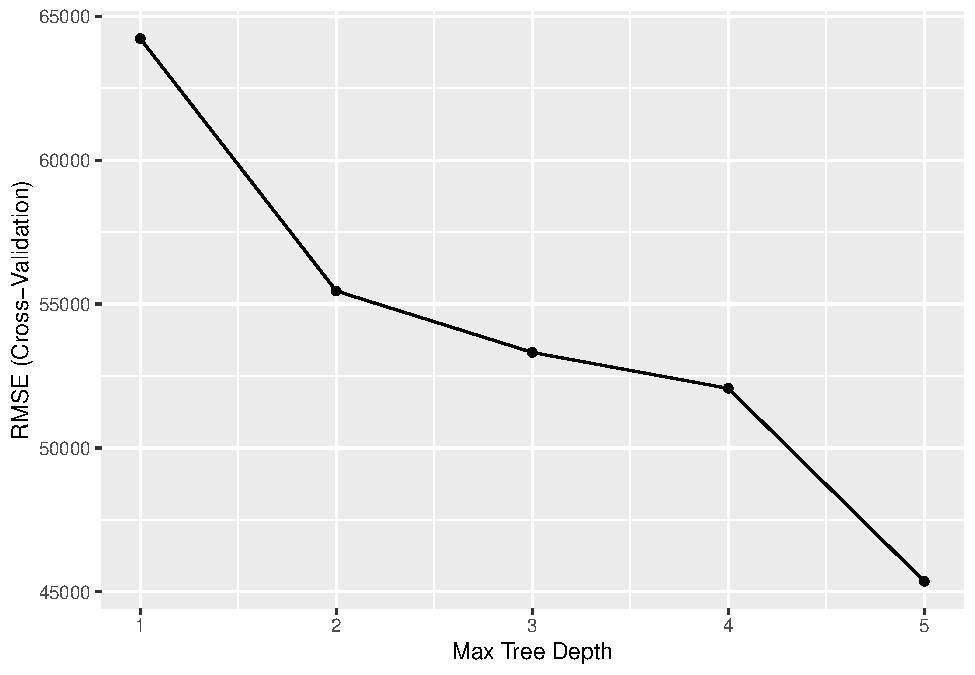
\includegraphics{LAB02_files/figure-latex/unnamed-chunk-6-1.pdf}

\begin{Shaded}
\begin{Highlighting}[]
\NormalTok{test.cart  }\OtherTok{\textless{}{-}} \FunctionTok{predict}\NormalTok{(train.cart, }\AttributeTok{newdata=}\NormalTok{test)}
\NormalTok{error.cart }\OtherTok{\textless{}{-}}\NormalTok{ test}\SpecialCharTok{$}\NormalTok{Sale\_Price}\SpecialCharTok{{-}}\NormalTok{test.cart }
\end{Highlighting}
\end{Shaded}

\hypertarget{random-forest}{%
\subsection{Random Forest}\label{random-forest}}

Random Forest se construye utilizando los principios fundamentales de
los árboles de regresión y el bagging. Este úlimo, genera múltiples
muestras de los datos y las agrega a los múltiples árboles de regresión.
Pero al construir estos árboles de decisión se debe elegir una muestra
aleatoria de predictores\(X\) (llamados \(mtry\)).Esta agregación reduce
la variación del procedimiento general y da como resultado un mejor
rendimiento predictivo.

\begin{Shaded}
\begin{Highlighting}[]
\DocumentationTok{\#\#\# Ejecutar Random Forest}
\NormalTok{train.randomf }\OtherTok{\textless{}{-}} \FunctionTok{train}\NormalTok{(Sale\_Price }\SpecialCharTok{\textasciitilde{}}\NormalTok{ Year\_Built}\SpecialCharTok{+}\NormalTok{Gr\_Liv\_Area}\SpecialCharTok{+}\NormalTok{Roof\_Style}\SpecialCharTok{+}\NormalTok{Heating\_QC, }
                       \AttributeTok{data=}\NormalTok{train, }\AttributeTok{method=}\StringTok{"rf"}\NormalTok{,  }
                       \AttributeTok{trControl =} \FunctionTok{trainControl}\NormalTok{(}\StringTok{"cv"}\NormalTok{, }\AttributeTok{number=}\DecValTok{5}\NormalTok{),}
                       \AttributeTok{preProcess =} \FunctionTok{c}\NormalTok{(}\StringTok{"center"}\NormalTok{,}\StringTok{"scale"}\NormalTok{),}
                       \AttributeTok{tuneLength =} \DecValTok{5} 
\NormalTok{)}
\FunctionTok{print}\NormalTok{(train.randomf)}
\end{Highlighting}
\end{Shaded}

\begin{verbatim}
## Random Forest 
## 
## 2051 samples
##    4 predictor
## 
## Pre-processing: centered (11), scaled (11) 
## Resampling: Cross-Validated (5 fold) 
## Summary of sample sizes: 1641, 1640, 1641, 1641, 1641 
## Resampling results across tuning parameters:
## 
##   mtry  RMSE   Rsquared  MAE  
##    2    48138  0.706     32177
##    4    40339  0.756     26781
##    6    38848  0.767     25656
##    8    39065  0.764     25935
##   11    39689  0.757     26369
## 
## RMSE was used to select the optimal model using the smallest value.
## The final value used for the model was mtry = 6.
\end{verbatim}

\begin{Shaded}
\begin{Highlighting}[]
\FunctionTok{ggplot}\NormalTok{(train.randomf)}
\end{Highlighting}
\end{Shaded}

\includegraphics{LAB02_files/figure-latex/unnamed-chunk-7-1.pdf}

\begin{Shaded}
\begin{Highlighting}[]
\NormalTok{test.randomf  }\OtherTok{\textless{}{-}} \FunctionTok{predict}\NormalTok{(train.randomf, }\AttributeTok{newdata=}\NormalTok{test) }
\NormalTok{error.randomf }\OtherTok{\textless{}{-}}\NormalTok{ test}\SpecialCharTok{$}\NormalTok{Sale\_Price}\SpecialCharTok{{-}}\NormalTok{test.randomf}
\end{Highlighting}
\end{Shaded}

\hypertarget{comparaciuxf3n-de-modelos}{%
\subsection{Comparación de modelos}\label{comparaciuxf3n-de-modelos}}

\begin{Shaded}
\begin{Highlighting}[]
\NormalTok{sales.test }\OtherTok{\textless{}{-}} \FunctionTok{data.frame}\NormalTok{(}\AttributeTok{lm=}\NormalTok{test.lm, }\AttributeTok{mars=}\FunctionTok{unname}\NormalTok{(test.mars),  }\AttributeTok{knn=}\NormalTok{test.knn,  }\AttributeTok{cart=}\NormalTok{test.cart,  }\AttributeTok{rf=}\NormalTok{test.randomf, }\AttributeTok{sales=}\NormalTok{test}\SpecialCharTok{$}\NormalTok{Sale\_Price)}
\NormalTok{error.test }\OtherTok{\textless{}{-}} \FunctionTok{data.frame}\NormalTok{(}\AttributeTok{lm=}\NormalTok{error.lm, }\AttributeTok{mars=}\FunctionTok{unname}\NormalTok{(error.mars), }\AttributeTok{knn=}\NormalTok{error.knn, }\AttributeTok{cart=}\NormalTok{error.cart, }\AttributeTok{rf=}\NormalTok{error.randomf)}

\FunctionTok{summary}\NormalTok{(}\FunctionTok{abs}\NormalTok{(error.test))}
\end{Highlighting}
\end{Shaded}

\begin{verbatim}
##        lm              mars             knn              cart       
##  Min.   :    31   Min.   :   133   Min.   :     9   Min.   :    13  
##  1st Qu.:  9891   1st Qu.: 10146   1st Qu.:  8000   1st Qu.: 10387  
##  Median : 22802   Median : 21413   Median : 19077   Median : 23566  
##  Mean   : 30386   Mean   : 28767   Mean   : 27700   Mean   : 32816  
##  3rd Qu.: 40731   3rd Qu.: 37686   3rd Qu.: 36841   3rd Qu.: 43279  
##  Max.   :475711   Max.   :444038   Max.   :306721   Max.   :276079  
##        rf        
##  Min.   :    47  
##  1st Qu.:  7455  
##  Median : 17461  
##  Mean   : 25058  
##  3rd Qu.: 33158  
##  Max.   :279300
\end{verbatim}

\begin{Shaded}
\begin{Highlighting}[]
\FunctionTok{summary}\NormalTok{(error.test)}
\end{Highlighting}
\end{Shaded}

\begin{verbatim}
##        lm               mars              knn               cart        
##  Min.   :-475711   Min.   :-444038   Min.   :-306721   Min.   :-235019  
##  1st Qu.: -26428   1st Qu.: -24660   1st Qu.: -23082   1st Qu.: -30352  
##  Median :  -3344   Median :  -2154   Median :  -3282   Median :  -4574  
##  Mean   :  -3070   Mean   :  -2542   Mean   :  -2287   Mean   :  -3593  
##  3rd Qu.:  18394   3rd Qu.:  18052   3rd Qu.:  14475   3rd Qu.:  18398  
##  Max.   : 212784   Max.   : 207689   Max.   : 258964   Max.   : 276079  
##        rf         
##  Min.   :-279300  
##  1st Qu.: -21392  
##  Median :  -4189  
##  Mean   :  -2688  
##  3rd Qu.:  11949  
##  Max.   : 193366
\end{verbatim}

\begin{Shaded}
\begin{Highlighting}[]
\FunctionTok{boxplot}\NormalTok{(}\FunctionTok{abs}\NormalTok{(}\FunctionTok{subset}\NormalTok{(error.test, }\AttributeTok{select=}\SpecialCharTok{{-}}\NormalTok{lm))); }\FunctionTok{title}\NormalTok{(}\AttributeTok{main=}\StringTok{"ML models"}\NormalTok{, }\AttributeTok{sub=}\StringTok{"Forecasting Absolute Errors"}\NormalTok{)}
\end{Highlighting}
\end{Shaded}

\includegraphics{LAB02_files/figure-latex/unnamed-chunk-8-1.pdf}

\begin{Shaded}
\begin{Highlighting}[]
\FunctionTok{boxplot}\NormalTok{(}\FunctionTok{subset}\NormalTok{(error.test, }\AttributeTok{select=}\SpecialCharTok{{-}}\NormalTok{lm)); }\FunctionTok{title}\NormalTok{(}\AttributeTok{main=}\StringTok{"ML models"}\NormalTok{, }\AttributeTok{sub=}\StringTok{"Forecasting Errors"}\NormalTok{)}
\end{Highlighting}
\end{Shaded}

\includegraphics{LAB02_files/figure-latex/unnamed-chunk-8-2.pdf}

\hypertarget{preguntas}{%
\subsection{Preguntas}\label{preguntas}}

\hypertarget{pregunta-1}{%
\subsubsection{Pregunta 1}\label{pregunta-1}}

Para esta pregunta se escogen atributos 10 (variables explicativas) que
puedan ser predictoras del precio de las casa. Se escogen entonces
\emph{Street, Lot\_Shape, Exter\_Cond, Central\_Air, Garage\_Area,
Kitchen\_Qual, Year\_Built, Gr\_Liv\_Area, Roof\_Style} y
\emph{Heating\_QC}.

¿ Por qué podrían ser útiles \emph{Garage\_Area, Kitchen\_Qual} y
\emph{Exter\_Cond}?

\begin{itemize}
\item
  \emph{Garage\_Area}: El sólo hecho de que una casa cuente con un
  garage suele implicar que la casa tenga un alto precio. Es necesario
  que esta sea de un tamaño considerable (en la mayoría de los casos en
  USA) para contar con un garage. En cuanto al área de este, mientras
  mayor es, significa que tiene capacidad para más vehículos (u otros
  objetos), lo que implica que la casa también debe ser mayor para poder
  dar el paso a un garage de mayor tamaño. Dicho esto, es esperable que
  a mayor área de garage, el precio de las casas sea mayor.
\item
  \emph{Kitchen\_Qual}: \emph{Este atributo es similar al anterior en el
  sentido de que una mayor calidad en la cocina implica que está
  apuntando a personas de mayores recursos, no a personas que sólo
  buscan una casa con cocina funcional, por lo que puede esperarce que a
  mayor calidad en la cocina, mayor sea el precio de la casa.}
\item
  \emph{Exter\_Cond}: Si la condición actual de la parte exterior de la
  casa no es óptima, es esperable que los precios de las casas sean
  menores, mientras que en una condición óptima sean mayores, ya que
  está directamente relacioando con la calidad de lo que se está
  comprando y no se pagarán precios altos por algo de mala calidad.
\end{itemize}

\begin{Shaded}
\begin{Highlighting}[]
\CommentTok{\# Construcción de la sub{-}base}

\NormalTok{Casas }\OtherTok{\textless{}{-}}\NormalTok{ Casas[,}\FunctionTok{c}\NormalTok{(}\StringTok{"Sale\_Price"}\NormalTok{, }\StringTok{"Street"}\NormalTok{, }\StringTok{"Lot\_Shape"}\NormalTok{, }\StringTok{"Exter\_Cond"}\NormalTok{, }\StringTok{"Central\_Air"}\NormalTok{, }\StringTok{"Garage\_Area"}\NormalTok{, }\StringTok{"Kitchen\_Qual"}\NormalTok{, }\StringTok{"Year\_Built"}\NormalTok{, }\StringTok{"Gr\_Liv\_Area"}\NormalTok{, }\StringTok{"Roof\_Style"}\NormalTok{, }\StringTok{"Heating\_QC"}\NormalTok{)]}

\CommentTok{\# Para evitar problemas pasamos los atributos de tipo}
\CommentTok{\# categóricos a factores}
\ControlFlowTok{for}\NormalTok{ (col }\ControlFlowTok{in} \FunctionTok{colnames}\NormalTok{(Casas))\{}
  \CommentTok{\# Si no forma parte de los numéricos }
  \ControlFlowTok{if}\NormalTok{ (}\SpecialCharTok{!}\NormalTok{col }\SpecialCharTok{\%in\%} \FunctionTok{c}\NormalTok{(}\StringTok{"Garage\_Area"}\NormalTok{, }\StringTok{"Gr\_Liv\_Area"}\NormalTok{, }\StringTok{"Year\_Built"}\NormalTok{))\{}
\NormalTok{    Casas[[col]] }\OtherTok{\textless{}{-}} \FunctionTok{as.factor}\NormalTok{(Casas[[col]])}
\NormalTok{  \}}
\NormalTok{\}}

\CommentTok{\# Pasamos la variable dependiente (Sales Prices) a numerica}
\NormalTok{Casas}\SpecialCharTok{$}\NormalTok{Sale\_Price }\OtherTok{=} \FunctionTok{as.numeric}\NormalTok{(Casas}\SpecialCharTok{$}\NormalTok{Sale\_Price)}

\CommentTok{\# Tampoco tiene sentido el año numéricamente, pero son demasiados factores para analizarlo como tal. Por ende, vamos a transformar este atrbibuto a la distancia entre el último año en la base con la columna en cuestión, con lo que tendremos una diferencia de años que sí tiene sentido numéricamente para comparar}
\NormalTok{Casas}\SpecialCharTok{$}\NormalTok{Year\_Built }\OtherTok{\textless{}{-}} \FunctionTok{max}\NormalTok{(Casas}\SpecialCharTok{$}\NormalTok{Year\_Built) }\SpecialCharTok{{-}}\NormalTok{ Casas}\SpecialCharTok{$}\NormalTok{Year\_Built}

\CommentTok{\# Vemos las descripciones de los atributos}
\FunctionTok{str}\NormalTok{(Casas)}
\end{Highlighting}
\end{Shaded}

\begin{verbatim}
## 'data.frame':    2930 obs. of  11 variables:
##  $ Sale_Price  : num  635 139 451 724 538 561 630 544 704 536 ...
##  $ Street      : Factor w/ 2 levels "Grvl","Pave": 2 2 2 2 2 2 2 2 2 2 ...
##  $ Lot_Shape   : Factor w/ 4 levels "Irregular","Moderately_Irregular",..: 4 3 4 3 4 4 3 4 4 3 ...
##  $ Exter_Cond  : Factor w/ 5 levels "Excellent","Fair",..: 5 5 5 5 5 5 5 5 5 5 ...
##  $ Central_Air : Factor w/ 2 levels "N","Y": 2 2 2 2 2 2 2 2 2 2 ...
##  $ Garage_Area : int  528 730 312 522 482 470 582 506 608 442 ...
##  $ Kitchen_Qual: Factor w/ 5 levels "Excellent","Fair",..: 5 5 3 1 5 3 3 3 3 3 ...
##  $ Year_Built  : int  50 49 52 42 13 12 9 18 15 11 ...
##  $ Gr_Liv_Area : int  1656 896 1329 2110 1629 1604 1338 1280 1616 1804 ...
##  $ Roof_Style  : Factor w/ 6 levels "Flat","Gable",..: 4 2 4 4 2 2 2 2 2 2 ...
##  $ Heating_QC  : Factor w/ 5 levels "Excellent","Fair",..: 2 5 5 1 3 1 1 1 1 3 ...
\end{verbatim}

\begin{Shaded}
\begin{Highlighting}[]
\CommentTok{\# samples aleatorio}
\NormalTok{index }\OtherTok{\textless{}{-}} \FunctionTok{sample}\NormalTok{(}\DecValTok{1}\SpecialCharTok{:}\FunctionTok{nrow}\NormalTok{(Casas), }\AttributeTok{size=} \FunctionTok{nrow}\NormalTok{(Casas)}\SpecialCharTok{*}\FloatTok{0.7}\NormalTok{)}

\CommentTok{\# entrenamiento 70\%}
\NormalTok{train }\OtherTok{\textless{}{-}}\NormalTok{ Casas[index, ]}
\CommentTok{\# test 30\%}
\NormalTok{test  }\OtherTok{\textless{}{-}}\NormalTok{ Casas[}\SpecialCharTok{{-}}\NormalTok{index, ]}
\end{Highlighting}
\end{Shaded}

\hypertarget{pregunta-2}{%
\subsubsection{Pregunta 2}\label{pregunta-2}}

A continuación se emplean 3 modelos de predicción: regresión lineal, knn
y random forest. Para estos se utiliza una base de entrenamiento con el
70\% de la base de datos, con las que se obtendrán los parámetros de los
modelos para posteriormente realizar una predicción del precio de venta
sobre la base de testeo (30\% de los datos).

\hypertarget{regresiuxf3n-lineal-1}{%
\subparagraph{Regresión Lineal}\label{regresiuxf3n-lineal-1}}

\begin{Shaded}
\begin{Highlighting}[]
\CommentTok{\#Corra 1 modelo de regresión lineal y 2 modelos de Machine Learning vistos en la clase con la base de datos reducida,  para predecir el precio de las casas.}

\NormalTok{train.lm }\OtherTok{\textless{}{-}} \FunctionTok{train}\NormalTok{(}\AttributeTok{form =}\NormalTok{ Sale\_Price }\SpecialCharTok{\textasciitilde{}}\NormalTok{ ., }\CommentTok{\#Fórmula}
  \AttributeTok{data =}\NormalTok{ train, }\CommentTok{\#Datos}
  \AttributeTok{method =} \StringTok{"lm"}\NormalTok{, }\CommentTok{\#Algoritmo }
  \AttributeTok{trControl =} \FunctionTok{trainControl}\NormalTok{(}\AttributeTok{method =} \StringTok{"cv"}\NormalTok{, }\AttributeTok{number =} \DecValTok{5}\NormalTok{) }\CommentTok{\#Method = cross validation, number=10 (k{-}fold) }
\NormalTok{)}
\end{Highlighting}
\end{Shaded}

\begin{verbatim}
## Warning in predict.lm(modelFit, newdata): prediction from a rank-deficient fit
## may be misleading
\end{verbatim}

\begin{Shaded}
\begin{Highlighting}[]
\FunctionTok{print}\NormalTok{(train.lm)}
\end{Highlighting}
\end{Shaded}

\begin{verbatim}
## Linear Regression 
## 
## 2051 samples
##   10 predictor
## 
## No pre-processing
## Resampling: Cross-Validated (5 fold) 
## Summary of sample sizes: 1641, 1640, 1641, 1642, 1640 
## Resampling results:
## 
##   RMSE  Rsquared  MAE 
##   115   0.795     82.6
## 
## Tuning parameter 'intercept' was held constant at a value of TRUE
\end{verbatim}

\begin{Shaded}
\begin{Highlighting}[]
\NormalTok{test.lm  }\OtherTok{\textless{}{-}} \FunctionTok{predict}\NormalTok{(train.lm, }\AttributeTok{newdata=}\NormalTok{test) }
\NormalTok{error.lm }\OtherTok{\textless{}{-}}\NormalTok{ test}\SpecialCharTok{$}\NormalTok{Sale\_Price}\SpecialCharTok{{-}}\NormalTok{test.lm}
\end{Highlighting}
\end{Shaded}

\hypertarget{knn}{%
\subparagraph{KNN}\label{knn}}

\begin{Shaded}
\begin{Highlighting}[]
\DocumentationTok{\#\#\# Ejecutar KNN}
\NormalTok{train.knn }\OtherTok{\textless{}{-}} \FunctionTok{train}\NormalTok{(Sale\_Price }\SpecialCharTok{\textasciitilde{}}\NormalTok{ ., }
                   \AttributeTok{data=}\NormalTok{train, }\AttributeTok{method=}\StringTok{"knn"}\NormalTok{,  }
                   \AttributeTok{trControl =} \FunctionTok{trainControl}\NormalTok{(}\StringTok{"cv"}\NormalTok{, }\AttributeTok{number=}\DecValTok{5}\NormalTok{),}
                   \AttributeTok{preProcess =} \FunctionTok{c}\NormalTok{(}\StringTok{"center"}\NormalTok{,}\StringTok{"scale"}\NormalTok{),}
                   \AttributeTok{tuneLength =} \DecValTok{5} 
\NormalTok{)}
\end{Highlighting}
\end{Shaded}

\begin{verbatim}
## Warning in preProcess.default(thresh = 0.95, k = 5, freqCut = 19, uniqueCut =
## 10, : These variables have zero variances: Kitchen_QualPoor

## Warning in preProcess.default(thresh = 0.95, k = 5, freqCut = 19, uniqueCut =
## 10, : These variables have zero variances: Kitchen_QualPoor

## Warning in preProcess.default(thresh = 0.95, k = 5, freqCut = 19, uniqueCut =
## 10, : These variables have zero variances: Kitchen_QualPoor

## Warning in preProcess.default(thresh = 0.95, k = 5, freqCut = 19, uniqueCut =
## 10, : These variables have zero variances: Kitchen_QualPoor

## Warning in preProcess.default(thresh = 0.95, k = 5, freqCut = 19, uniqueCut =
## 10, : These variables have zero variances: Kitchen_QualPoor
\end{verbatim}

\begin{Shaded}
\begin{Highlighting}[]
\FunctionTok{print}\NormalTok{(train.knn)}
\end{Highlighting}
\end{Shaded}

\begin{verbatim}
## k-Nearest Neighbors 
## 
## 2051 samples
##   10 predictor
## 
## Pre-processing: centered (25), scaled (25) 
## Resampling: Cross-Validated (5 fold) 
## Summary of sample sizes: 1639, 1640, 1642, 1642, 1641 
## Resampling results across tuning parameters:
## 
##   k   RMSE  Rsquared  MAE 
##    5  120   0.773     89.0
##    7  121   0.769     89.3
##    9  121   0.768     89.6
##   11  122   0.763     90.4
##   13  122   0.764     90.6
## 
## RMSE was used to select the optimal model using the smallest value.
## The final value used for the model was k = 5.
\end{verbatim}

\begin{Shaded}
\begin{Highlighting}[]
\FunctionTok{ggplot}\NormalTok{(train.knn)}
\end{Highlighting}
\end{Shaded}

\includegraphics{LAB02_files/figure-latex/unnamed-chunk-10-1.pdf}

\begin{Shaded}
\begin{Highlighting}[]
\NormalTok{test.knn  }\OtherTok{\textless{}{-}} \FunctionTok{predict}\NormalTok{(train.knn, }\AttributeTok{newdata=}\NormalTok{test) }
\NormalTok{error.knn }\OtherTok{\textless{}{-}}\NormalTok{ test}\SpecialCharTok{$}\NormalTok{Sale\_Price}\SpecialCharTok{{-}}\NormalTok{test.knn}
\end{Highlighting}
\end{Shaded}

\hypertarget{random-forest-1}{%
\subparagraph{Random Forest}\label{random-forest-1}}

\begin{Shaded}
\begin{Highlighting}[]
\DocumentationTok{\#\#\# Ejecutar Random Forest}
\NormalTok{train.randomf }\OtherTok{\textless{}{-}} \FunctionTok{train}\NormalTok{(Sale\_Price }\SpecialCharTok{\textasciitilde{}}\NormalTok{ Year\_Built}\SpecialCharTok{+}\NormalTok{Gr\_Liv\_Area}\SpecialCharTok{+}\NormalTok{Roof\_Style}\SpecialCharTok{+}\NormalTok{Heating\_QC, }
                       \AttributeTok{data=}\NormalTok{train, }\AttributeTok{method=}\StringTok{"rf"}\NormalTok{,  }
                       \AttributeTok{trControl =} \FunctionTok{trainControl}\NormalTok{(}\StringTok{"cv"}\NormalTok{, }\AttributeTok{number=}\DecValTok{5}\NormalTok{),}
                       \AttributeTok{preProcess =} \FunctionTok{c}\NormalTok{(}\StringTok{"center"}\NormalTok{,}\StringTok{"scale"}\NormalTok{),}
                       \AttributeTok{tuneLength =} \DecValTok{5} 
\NormalTok{)}
\end{Highlighting}
\end{Shaded}

\begin{verbatim}
## Warning in preProcess.default(thresh = 0.95, k = 5, freqCut = 19, uniqueCut =
## 10, : These variables have zero variances: Heating_QCPoor

## Warning in preProcess.default(thresh = 0.95, k = 5, freqCut = 19, uniqueCut =
## 10, : These variables have zero variances: Heating_QCPoor

## Warning in preProcess.default(thresh = 0.95, k = 5, freqCut = 19, uniqueCut =
## 10, : These variables have zero variances: Heating_QCPoor

## Warning in preProcess.default(thresh = 0.95, k = 5, freqCut = 19, uniqueCut =
## 10, : These variables have zero variances: Heating_QCPoor

## Warning in preProcess.default(thresh = 0.95, k = 5, freqCut = 19, uniqueCut =
## 10, : These variables have zero variances: Heating_QCPoor
\end{verbatim}

\begin{Shaded}
\begin{Highlighting}[]
\FunctionTok{print}\NormalTok{(train.randomf)}
\end{Highlighting}
\end{Shaded}

\begin{verbatim}
## Random Forest 
## 
## 2051 samples
##    4 predictor
## 
## Pre-processing: centered (11), scaled (11) 
## Resampling: Cross-Validated (5 fold) 
## Summary of sample sizes: 1641, 1641, 1640, 1641, 1641 
## Resampling results across tuning parameters:
## 
##   mtry  RMSE  Rsquared  MAE  
##    2    143   0.733     115.3
##    4    119   0.782      91.2
##    6    116   0.789      86.2
##    8    117   0.783      86.3
##   11    119   0.776      87.3
## 
## RMSE was used to select the optimal model using the smallest value.
## The final value used for the model was mtry = 6.
\end{verbatim}

\begin{Shaded}
\begin{Highlighting}[]
\FunctionTok{ggplot}\NormalTok{(train.randomf)}
\end{Highlighting}
\end{Shaded}

\includegraphics{LAB02_files/figure-latex/unnamed-chunk-11-1.pdf}

\begin{Shaded}
\begin{Highlighting}[]
\NormalTok{test.randomf  }\OtherTok{\textless{}{-}} \FunctionTok{predict}\NormalTok{(train.randomf, }\AttributeTok{newdata=}\NormalTok{test) }
\NormalTok{error.randomf }\OtherTok{\textless{}{-}}\NormalTok{ test}\SpecialCharTok{$}\NormalTok{Sale\_Price}\SpecialCharTok{{-}}\NormalTok{test.randomf}
\end{Highlighting}
\end{Shaded}

\hypertarget{pregunta-3}{%
\subsubsection{Pregunta 3}\label{pregunta-3}}

\begin{Shaded}
\begin{Highlighting}[]
\CommentTok{\# Comparación de Modelos: Compare los modelos a través de métricas presentadas en el laboratorio. }
\CommentTok{\# ¿Cuál es el mejor modelo predictivo?}

\NormalTok{sales.test }\OtherTok{\textless{}{-}} \FunctionTok{data.frame}\NormalTok{(}\AttributeTok{lm=}\NormalTok{test.lm, }\AttributeTok{knn=}\NormalTok{test.knn,  }\AttributeTok{rf=}\NormalTok{test.randomf, }\AttributeTok{sales=}\NormalTok{test}\SpecialCharTok{$}\NormalTok{Sale\_Price)}
\NormalTok{error.test }\OtherTok{\textless{}{-}} \FunctionTok{data.frame}\NormalTok{(}\AttributeTok{lm=}\NormalTok{error.lm, }\AttributeTok{knn=}\NormalTok{error.knn, }\AttributeTok{rf=}\NormalTok{error.randomf)}

\FunctionTok{summary}\NormalTok{(}\FunctionTok{abs}\NormalTok{(error.test))}
\end{Highlighting}
\end{Shaded}

\begin{verbatim}
##        lm           knn            rf     
##  Min.   :  1   Min.   :  0   Min.   :  0  
##  1st Qu.: 29   1st Qu.: 26   1st Qu.: 30  
##  Median : 65   Median : 61   Median : 63  
##  Mean   : 80   Mean   : 82   Mean   : 84  
##  3rd Qu.:110   3rd Qu.:118   3rd Qu.:120  
##  Max.   :559   Max.   :510   Max.   :436
\end{verbatim}

\begin{Shaded}
\begin{Highlighting}[]
\FunctionTok{summary}\NormalTok{(error.test)}
\end{Highlighting}
\end{Shaded}

\begin{verbatim}
##        lm            knn             rf      
##  Min.   :-559   Min.   :-445   Min.   :-436  
##  1st Qu.: -72   1st Qu.: -66   1st Qu.: -69  
##  Median : -10   Median :  -6   Median :  -7  
##  Mean   :  -6   Mean   :  -3   Mean   :  -2  
##  3rd Qu.:  55   3rd Qu.:  54   3rd Qu.:  59  
##  Max.   : 468   Max.   : 510   Max.   : 410
\end{verbatim}

\begin{Shaded}
\begin{Highlighting}[]
\FunctionTok{boxplot}\NormalTok{(}\FunctionTok{abs}\NormalTok{(}\FunctionTok{subset}\NormalTok{(error.test))); }\FunctionTok{title}\NormalTok{(}\AttributeTok{main=}\StringTok{"ML models"}\NormalTok{, }\AttributeTok{sub=}\StringTok{"Forecasting Absolute Errors"}\NormalTok{)}
\end{Highlighting}
\end{Shaded}

\includegraphics{LAB02_files/figure-latex/p3-1.pdf}

\begin{Shaded}
\begin{Highlighting}[]
\FunctionTok{boxplot}\NormalTok{(}\FunctionTok{subset}\NormalTok{(error.test)); }\FunctionTok{title}\NormalTok{(}\AttributeTok{main=}\StringTok{"ML models"}\NormalTok{, }\AttributeTok{sub=}\StringTok{"Forecasting Errors"}\NormalTok{)}
\end{Highlighting}
\end{Shaded}

\includegraphics{LAB02_files/figure-latex/p3-2.pdf}

\textbf{¿Cuál es el mejor modelo predictivo?}

Observando los errores absolutos se puede observar que si bien todos los
valores son relativamente cercanos, el que presenta un menor error es el
modelo de regresión lineal simple (MAE = 80), seguido por el modelo KNN
(MAE = 82{]}), siendo el peor, pero con \textbf{muy baja diferencia}, el
random forest (MAE = 84).

\end{document}
